% !TeX program = xelatex
% 编译：xelatex C1_FlashKDA_汇报.tex（建议运行两次）
% 比例：16:9；建议汇报时长：10--12 分钟

\documentclass[aspectratio=169,10pt]{beamer}

\usepackage[UTF8]{ctex}
\usepackage{amsmath,amssymb}
\usepackage{booktabs}
\usepackage{array}
\usepackage{graphicx}
\usepackage{tikz}
\usetikzlibrary{arrows.meta,positioning,shapes.geometric,calc}

% ---------- 配色与版式 ----------
\definecolor{KdaNavy}{HTML}{0B1F33}
\definecolor{KdaBlue}{HTML}{1769AA}
\definecolor{KdaCyan}{HTML}{25A7B8}
\definecolor{KdaGreen}{HTML}{17845B}
\definecolor{KdaOrange}{HTML}{E27A32}
\definecolor{KdaRed}{HTML}{C23B3B}
\definecolor{KdaLight}{HTML}{F2F6FA}
\definecolor{KdaGray}{HTML}{5E6B75}

\setbeamercolor{normal text}{fg=KdaNavy,bg=white}
\setbeamercolor{structure}{fg=KdaBlue}
\setbeamercolor{frametitle}{fg=white,bg=KdaNavy}
\setbeamercolor{title}{fg=white}
\setbeamercolor{subtitle}{fg=white!82}
\setbeamercolor{author}{fg=white!90}
\setbeamercolor{date}{fg=white!75}
\setbeamercolor{block title}{fg=white,bg=KdaBlue}
\setbeamercolor{block body}{fg=KdaNavy,bg=KdaLight}
\setbeamercolor{alerted text}{fg=KdaRed}

\setbeamertemplate{navigation symbols}{}
\setbeamertemplate{itemize item}{\color{KdaCyan}$\blacktriangleright$}
\setbeamertemplate{itemize subitem}{\color{KdaBlue}$\bullet$}
\setbeamertemplate{enumerate item}{\color{KdaBlue}\insertenumlabel.}
\setbeamertemplate{blocks}[rounded][shadow=false]

\setbeamertemplate{footline}{%
  \leavevmode%
  \hbox{%
    \begin{beamercolorbox}[wd=.74\paperwidth,ht=2.6ex,dp=1.1ex,leftskip=1em]{author in head/foot}%
      \color{KdaGray}\scriptsize C1 FlashKDA：官方 kernel 为什么停在 SM80 MMA
    \end{beamercolorbox}%
    \begin{beamercolorbox}[wd=.26\paperwidth,ht=2.6ex,dp=1.1ex,rightskip=1em plus1fil]{date in head/foot}%
      \color{KdaGray}\scriptsize \insertframenumber\,/\,\inserttotalframenumber
    \end{beamercolorbox}%
  }%
}

\setbeamerfont{frametitle}{series=\bfseries,size=\large}
\setbeamerfont{title}{series=\bfseries,size=\LARGE}
\setbeamerfont{subtitle}{size=\large}

\newcommand{\good}[1]{\textcolor{KdaGreen}{\ifmmode\boldsymbol{#1}\else\textbf{#1}\fi}}
\newcommand{\bad}[1]{\textcolor{KdaRed}{\ifmmode\boldsymbol{#1}\else\textbf{#1}\fi}}
\newcommand{\key}[1]{\textcolor{KdaBlue}{\ifmmode\boldsymbol{#1}\else\textbf{#1}\fi}}
\newcommand{\code}[1]{\texttt{#1}}
\newcommand{\source}[1]{\vfill\hfill{\tiny\color{KdaGray}证据：#1}}

\title{C1 FlashKDA：官方 kernel 为什么停在 SM80 MMA}
\subtitle{B300 复现、瓶颈量化与 SM100 tcgen05 挑战}
\author{Assignment 02 · Team C1}
\date{2026}

\begin{document}

% ============================================================
% 1. 标题页（约 15 秒）
% ============================================================
{
\setbeamercolor{background canvas}{bg=KdaNavy}
\begin{frame}[plain]
  \titlepage
  \vspace{-0.5em}
  \begin{center}
    \color{KdaCyan}\rule{0.62\paperwidth}{1.2pt}

    \vspace{0.7em}
    \color{white!82}\small
    从“新指令应该更快”的直觉，走到“形状与依赖决定性能”的实证结论
  \end{center}
  \note{
    开场：题目观察到 FlashKDA 在 GB200/B300 上仍然执行 SM80 世代的 MMA。
    我们的目标是量化这个决定，或者用实验推翻它。
  }
\end{frame}
}

% ============================================================
% 2. 问题和答案（约 40 秒）
% ============================================================
\begin{frame}{研究问题与最终答案}
  \begin{block}{核心问题}
    对 \code{CHUNK=16}、小矩阵密集、chunk 间带状态依赖的 FlashKDA，
    在 B300 上把 SM80 \code{mma.sync} 直接换成 SM100 \code{tcgen05}，是否更快？
  \end{block}

  \vspace{0.15em}
  \scriptsize
  \begin{columns}[T,onlytextwidth]
    \column{0.49\textwidth}
      \textbf{直觉}
      \begin{itemize}
        \item B300 支持更新的 tensor-core 指令
        \item tcgen05 有 TMEM 和更强峰值能力
        \item “新指令”似乎应该替代“旧指令”
      \end{itemize}
    \column{0.49\textwidth}
      \textbf{实测答案}
      \begin{itemize}
        \item 正确性：\good{PASS}
        \item 原版：\key{1.755 ms}
        \item tcgen05 改版：\bad{17.552 ms}
        \item 改版约\bad{慢 10.001 倍}
      \end{itemize}
  \end{columns}

  \vspace{0.3em}
  \centering
  \large\bfseries 关键不是指令世代，而是算法粒度、物理 tile 与并行结构是否匹配。

  \note{
    先给结论，后面按“算法—推算—microbench—真实 kernel”的证据链解释。
    注意不要说 tcgen05 本身差，只说当前直接映射不合适。
  }
\end{frame}

% ============================================================
% 3. KDA 状态依赖（约 50 秒）
% ============================================================
\begin{frame}{KDA：8192 个 token 为什么不能全部打散？}
  \begin{columns}[T,onlytextwidth]
    \column{0.42\textwidth}
      \begin{block}{每个 head 的概念递推}
      \[
        S_t = d_t S_{t-1} + \Delta S_t,
        \qquad o_t = q_t S_t
      \]
      \end{block}
      \begin{itemize}
        \item 历史被压缩到 $D\times D$ 状态 $S$
        \item 同一 sequence、同一 head 的状态前后依赖
        \item FlashKDA 将序列分为长度 16 的 chunk
      \end{itemize}

    \column{0.56\textwidth}
      \centering
      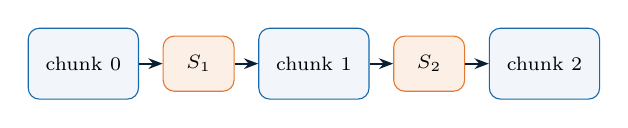
\begin{tikzpicture}[
        node distance=3mm,
        box/.style={draw=KdaBlue,rounded corners,minimum width=14mm,minimum height=9mm,fill=KdaLight,font=\scriptsize},
        state/.style={draw=KdaOrange,rounded corners,minimum width=9mm,minimum height=7mm,fill=KdaOrange!12,font=\scriptsize},
        arr/.style={-{Stealth[length=1.8mm]},thick,KdaNavy}
      ]
        \node[box] (c0) {chunk 0};
        \node[state,right=of c0] (s1) {$S_1$};
        \node[box,right=of s1] (c1) {chunk 1};
        \node[state,right=of c1] (s2) {$S_2$};
        \node[box,right=of s2] (c2) {chunk 2};
        \draw[arr] (c0)--(s1); \draw[arr] (s1)--(c1);
        \draw[arr] (c1)--(s2); \draw[arr] (s2)--(c2);
      \end{tikzpicture}

      \vspace{0.45em}
      \raggedright\scriptsize
      \textcolor{KdaGreen}{\textbf{可并行：}不同 sequence、不同 head、chunk 内计算}\par
      \textcolor{KdaRed}{\textbf{不可直接并行：}同一 sequence/head 的相邻状态更新}\par
      \vspace{0.4em}
      fixed $T=8192,H=96$：每条链有 $8192/16=512$ 个 chunk，
      K2 只有约 $1\times96=96$ 条独立链。
  \end{columns}

  \note{
    回答常见误解：不是 8192 token 完全不能并行；不能并行的是同一状态链的 chunk 更新。
    不同 head、不同 sequence 仍然独立。
  }
\end{frame}

% ============================================================
% 4. K1/K2 与项目结构（约 55 秒）
% ============================================================
\begin{frame}{从 Python 到 GPU：项目结构与执行链}
  \centering
  \begin{tikzpicture}[
    node distance=3.2mm,
    box/.style={draw=KdaBlue,rounded corners,minimum width=35mm,minimum height=6.2mm,fill=KdaLight,align=center,font=\small},
    gpu/.style={draw=KdaOrange,rounded corners,minimum width=42mm,minimum height=7mm,fill=KdaOrange!12,align=center,font=\small},
    arr/.style={-{Stealth[length=2mm]},thick,KdaNavy}
  ]
    \node[box] (py) {\code{flash\_kda.fwd()}\\Python 用户接口};
    \node[box,below=of py] (so) {\code{flash\_kda\_C.so}\\编译后的 C++/CUDA 扩展};
    \node[box,below=of so] (cpp) {\code{csrc/flash\_kda.cpp}\\参数检查与 pybind 导出};
    \node[box,below=of cpp] (launch) {\code{fwd\_launch.cu}\\模板选择与 kernel launch};
    \node[gpu,below left=4mm and 3mm of launch] (k1) {K1: \code{fwd\_kernel1.cuh}\\chunk-parallel prepare};
    \node[gpu,below right=4mm and 3mm of launch] (k2) {K2: \code{fwd\_kernel2.cuh}\\state recurrence};
    \draw[arr] (py)--(so); \draw[arr] (so)--(cpp); \draw[arr] (cpp)--(launch);
    \draw[arr] (launch)--(k1); \draw[arr] (launch)--(k2);
    \draw[-{Stealth[length=2mm]},thick,KdaCyan] (k1)--node[above,font=\scriptsize]{workspace}(k2);
  \end{tikzpicture}

  \vspace{0.4em}
  \begin{columns}[T,onlytextwidth]
    \column{0.49\textwidth}
      \textbf{原版：}
      \code{flash\_kda} $\rightarrow$ \code{flash\_kda\_C}
    \column{0.49\textwidth}
      \textbf{改版：}
      \code{flash\_kda\_tcgen05} $\rightarrow$ \code{flash\_kda\_tcgen05\_C}
  \end{columns}

  \vspace{0.05em}
  \centering\scriptsize
  两套包名允许在\key{同一进程、同一输入、同一张卡}上直接对拍。

  \note{
    flash\_kda 是 Python 包；flash\_kda\_C 是 setup.py 编译出来的动态库。
    Python 不是自己算 CUDA，而是通过 .so 启动 csrc 中的 GPU kernel。
  }
\end{frame}

% ============================================================
% 5. 复现 benchmark（约 45 秒）
% ============================================================
\begin{frame}{复现：B300 上 FlashKDA 仍然很快}
  \small
  \begin{center}
  \begin{tabular}{lrrrr}
    \toprule
    场景（$T=8192,H=96,D=128$） & FlashKDA & chunk\_kda & 对 chunk 加速 & 对 GDR 加速 \\
    \midrule
    fixed：$1\times8192$ & 1.0304 ms & 2.5793 ms & \good{2.503$\times$} & 1.255$\times$ \\
    varlen：6 条不等长 & 0.8598 ms & 2.6187 ms & \good{3.046$\times$} & 1.574$\times$ \\
    varlen：$8\times1024$ & 0.6998 ms & 2.5774 ms & \good{3.683$\times$} & 1.890$\times$ \\
    \bottomrule
  \end{tabular}
  \end{center}

  \vspace{0.6em}
  \begin{columns}[T,onlytextwidth]
    \column{0.48\textwidth}
      \begin{block}{复现可信度}
        B300 三个场景分别为 1.0304/0.8598/0.6998 ms，
        与官方 GB200 的 1.0087/0.8597/0.7064 ms 接近。
      \end{block}
    \column{0.48\textwidth}
      \begin{block}{状态链并行的直接证据}
        总 token 不变，$8\times1024$ 比 $1\times8192$ 快：
        \[
          1.0304/0.6998 = \good{1.472\times}
        \]
      \end{block}
  \end{columns}

  \source{FlashKDA/BENCHMARK\_GB200.md；B300 bench\_fwd.py 日志}
  \note{
    先说明原版并不慢：在 B300 上对 Triton chunk\_kda 仍有 2.5--3.68 倍优势。
    varlen 更快不是少算，而是独立状态链更多。
  }
\end{frame}

% ============================================================
% 6. CHUNK=16 三原因（约 60 秒）
% ============================================================
\begin{frame}{讨论 1：CHUNK=16 的三个约束}
  \begin{columns}[T,onlytextwidth]
    \column{0.32\textwidth}
      \begin{block}{1. 数值范围}
        最坏 $g_t=-5$：
        \[
          G_C=-5C
        \]
        \begin{tabular}{ccl}
          $C$ & $G_C$ & 结果 \\
          \hline
          16 & -80 & \good{尚安全} \\
          32 & -160 & \bad{溢出/下溢} \\
          64 & -320 & \bad{更严重}
        \end{tabular}
      \end{block}

    \column{0.32\textwidth}
      \begin{block}{2. Neumann 求逆}
        \[
          (I-L)^{-1}=\sum_{i=0}^{C-1}L^i
        \]
        每 token 求逆 FLOP：
        \begin{tabular}{cr}
          $C$ & 相对 16 \\
          \hline
          16 & 1.00$\times$ \\
          32 & \bad{5.33$\times$} \\
          64 & \bad{26.67$\times$}
        \end{tabular}
      \end{block}

    \column{0.32\textwidth}
      \begin{block}{3. 指令形状}
        SM80：
        \[
          \code{m16n8k16}
        \]
        \begin{itemize}
          \item M=16 正好匹配 chunk 行数
          \item 无需补到更大的物理 M
          \item 小 tile 固定成本低
        \end{itemize}
      \end{block}
  \end{columns}

  \vspace{0.4em}
  \centering\large
  \bad{最先破的是数值范围}；即使增加 rescale，求逆和资源代价仍明显上涨。

  \note{
    最坏 gate 累加：C16 是 -80，仍在 FP32/BF16 共同指数范围附近；
    C32 到 -160，需要分段 anchor/rescale，这已经是算法变化。
  }
\end{frame}

% ============================================================
% 7. tile 不匹配（约 55 秒）
% ============================================================
\begin{frame}{讨论 2：逻辑 M=16 遇到物理 M=128}
  \begin{columns}[T,onlytextwidth]
    \column{0.45\textwidth}
      \centering
      \begin{tikzpicture}[x=0.048cm,y=0.048cm]
        \fill[KdaGreen!75] (0,0) rectangle (128,16);
        \fill[KdaRed!18] (0,16) rectangle (128,128);
        \draw[very thick,KdaNavy] (0,0) rectangle (128,128);
        \draw[thick,KdaNavy] (0,16)--(128,16);
        \node[white,font=\bfseries] at (64,8) {有效逻辑行：16};
        \node[KdaRed,font=\bfseries,align=center] at (64,72) {补零行：112\\87.5\% 无效};
        \node[below,font=\small] at (64,-5) {tcgen05 物理 tile：$128\times128\times16$};
      \end{tikzpicture}

    \column{0.53\textwidth}
      \begin{itemize}
        \item 单个 M=16 GEMM：
        \[
          \text{issued/useful}=128/16=\bad{8\times}
        \]
        \item K2 每 chunk 动态发出 19 次 tcgen05：
        \begin{itemize}
          \item $kS^T$：8 次；$qS^T$：8 次
          \item $INV\cdot U$：1 次；$Mqk\cdot U$：1 次
          \item state delta：1 次（唯一自然 M=128）
        \end{itemize}
        \item 综合物理/有效行工作：
        \[
          \frac{19\cdot128}{18\cdot16+128}=\bad{5.846\times}
        \]
        \item 仅约 \good{17.1\%} 的物理行是有效计算
      \end{itemize}
  \end{columns}

  \note{
    这是最核心的一张图。注意说“本实验使用的 tcgen05 映射物理 M=128”，
    不要泛化成所有可能 tcgen05 用法都只能这样。
  }
\end{frame}

% ============================================================
% 8. microbench（约 45 秒）
% ============================================================
\begin{frame}{Microbench：纸面浪费能否在机器上观察到？}
  \small
  \begin{center}
  \begin{tabular}{lrrrr}
    \toprule
    形状 & SM80 MMA & tcgen05 & tcgen05/SM80 & issued/useful \\
    \midrule
    逻辑 M=16，补到 M=128 & 0.006155 ms & 0.012300 ms & \bad{0.500$\times$} & 8.0$\times$ \\
    自然 M=128 & 0.014542 ms & 0.050765 ms & \bad{0.286$\times$} & 1.0$\times$ \\
    \bottomrule
  \end{tabular}
  \end{center}

  \vspace{0.7em}
  \begin{columns}[T,onlytextwidth]
    \column{0.47\textwidth}
      \begin{block}{正确性}
        两组均：\good{PASS}，mismatches=0，max\_abs=0。
      \end{block}
    \column{0.49\textwidth}
      \begin{block}{为什么自然 M=128 仍可能慢？}
        问题很小且每次立刻同步读回，descriptor、TMEM、commit/wait 等固定成本没有被长流水摊薄。
      \end{block}
  \end{columns}

  \centering
  microbench 不是最终结论，而是决定是否值得接入真实 K2 的\key{中间证据}。

  \source{experiments/instruction\_only\_mma.cu；B300 run\_b300.sh 输出}
  \note{
    正确表达：它证明当前直接映射没有单指令级收益；最终仍需真实 kernel 验证。
  }
\end{frame}

% ============================================================
% 9. NCU（约 65 秒）
% ============================================================
\begin{frame}{讨论 4：不是简单的 compute-bound / memory-bound}
  \small
  \begin{center}
  \begin{tabular}{lrr}
    \toprule
    NCU 指标 & K1 prepare & fixed K2 recurrence \\
    \midrule
    Compute (SM) throughput & 70.21\% & 20.6--21.9\% \\
    DRAM throughput & 58.99\% & 18.6--19.6\% \\
    L2 throughput & 72.32\% & 27--28\% \\
    Achieved occupancy & \good{96.60\%} & \bad{9.37\%} \\
    Eligible warps/scheduler & 2.27 & \bad{0.34--0.36} \\
    No eligible & 28.55\% & \bad{约 67.5\%} \\
    Grid size & 49,152 & \bad{96} \\
    Dynamic shared/CTA & 21.25 KiB & 98.43 KiB \\
    \bottomrule
  \end{tabular}
  \end{center}

  \vspace{0.3em}
  \begin{columns}[T,onlytextwidth]
    \column{0.48\textwidth}
      \textbf{K1：}大量 chunk 独立，compute/cache/memory 都高，属于高吞吐混合阶段。
    \column{0.48\textwidth}
      \textbf{fixed K2：}计算和 HBM 都没打满；主因是\bad{低 CTA 数、状态依赖、同步和资源限制}。
  \end{columns}

  \vspace{0.4em}
  \centering
  varlen 从 6 条增至 8 条后，K2 Compute 从约 28\% 升至约 40\%，
  DRAM 从约 25\% 升至约 35\%：\key{独立状态链越多，GPU 越容易被填满。}

  \source{b300\_fixed/varlen\_h96\_run1\_details.txt}
  \note{
    重点：compute 20%、DRAM 19% 不是“平衡”，而是两边都没吃满。
    occupancy 和 eligible warp 揭示 latency/parallelism 才是主要问题。
  }
\end{frame}

% ============================================================
% 10. 并行候选（约 50 秒）
% ============================================================
\begin{frame}{讨论 3：状态有依赖，并行度还能从哪里来？}
  \small
  \begin{tabular}{>{\bfseries}p{0.18\textwidth}p{0.30\textwidth}p{0.36\textwidth}}
    \toprule
    候选方案 & 潜在收益 & 反例 / 风险 \\
    \midrule
    多 head 合一个 CTA
      & 填满 M=128，减少 padding
      & 每 head 状态约 32 KiB；CTA 变少，寄存器/共享内存压力增大 \\
    \addlinespace
    Persistent + work queue
      & 改善 varlen 长短不均和尾部效应
      & fixed N=1 时不能创造新状态链；原版 K2 已在 CTA 内循环 chunk \\
    \addlinespace
    2-CTA / cluster
      & 可切 D 维，流水 TMA/计算
      & 每 chunk 的 cluster barrier 位于关键路径，且资源翻倍 \\
    \addlinespace
    Affine prefix scan
      & 理论上打破 chunk 串行深度
      & 中间量、数值顺序和组合成本大，属于算法重写 \\
    \bottomrule
  \end{tabular}

  \vspace{0.6em}
  \centering
  \key{优先方向：}多序列/多 head 调度提高 useful tile；
  若要真正突破单链依赖，则需要算法级 scan/rescale。

  \note{
    这一页要体现“提出方案并互相找反例”。不要只列名字，必须说每个方案为何可能失败。
  }
\end{frame}

% ============================================================
% 11. 真实挑战（约 55 秒）
% ============================================================
\begin{frame}{挑战实现：不是玩具 GEMM，而是真实 K2}
  \begin{columns}[T,onlytextwidth]
    \column{0.48\textwidth}
      \begin{block}{保持不变}
        \begin{itemize}
          \item KDA 数学语义与 \code{CHUNK=16}
          \item K1/K2 两阶段和 chunk 顺序
          \item gate、beta、状态落盘点
          \item Python API 输入输出
        \end{itemize}
      \end{block}
      \begin{block}{只替换 K2 GEMM 路径}
        \begin{itemize}
          \item \code{fwd\_kernel2.cuh} 接入 tcgen05
          \item \code{tcgen05.cuh} 封装 PTX/TMEM/mbarrier
          \item K1 仍保留原版 HMMA
        \end{itemize}
      \end{block}

    \column{0.50\textwidth}
      \centering
      \begin{tikzpicture}[
        node distance=3.5mm,
        box/.style={draw=KdaBlue,rounded corners,minimum width=46mm,minimum height=6.5mm,fill=KdaLight,align=center,font=\scriptsize},
        tc/.style={draw=KdaOrange,rounded corners,minimum width=46mm,minimum height=6.5mm,fill=KdaOrange!12,align=center,font=\scriptsize},
        arr/.style={-{Stealth[length=1.8mm]},thick,KdaNavy}
      ]
        \node[box] (in) {K1 workspace + old state};
        \node[tc,below=of in] (ks) {8$\times$ tcgen05: $kS^T$};
        \node[tc,below=of ks] (qs) {8$\times$ tcgen05: $qS^T$};
        \node[box,below=of qs] (u0) {$U_0=(v-KS)\,\sigma(\beta)$};
        \node[tc,below=of u0] (small) {tcgen05: $INV\,U_0$ 与 $Mqk\,U$};
        \node[tc,below=of small] (delta) {tcgen05: $k^T U$（state delta）};
        \node[box,below=of delta] (out) {output + new state $\rightarrow$ next chunk};
        \draw[arr] (in)--(ks); \draw[arr] (ks)--(qs); \draw[arr] (qs)--(u0);
        \draw[arr] (u0)--(small); \draw[arr] (small)--(delta); \draw[arr] (delta)--(out);
      \end{tikzpicture}
  \end{columns}

  \note{
    experiments 是 microbench；FInal/FlashKDA-tcgen05 才是最终真实改版。
    本挑战范围是 K2，所以 K1 的 HMMA 保留是预期。
  }
\end{frame}

% ============================================================
% 12. 正确性（约 55 秒）
% ============================================================
\begin{frame}{正确性：为什么要四方对拍？}
  \small
  \begin{columns}[T,onlytextwidth]
    \column{0.36\textwidth}
      \resizebox{\linewidth}{!}{%
      \begin{tikzpicture}[
        node distance=4mm,
        box/.style={draw=KdaBlue,rounded corners,minimum width=34mm,minimum height=7mm,fill=KdaLight,align=center,font=\scriptsize},
        arr/.style={<->,thick,KdaCyan}
      ]
        \node[box] (new) {tcgen05 改版};
        \node[box,below=of new] (old) {原版 FlashKDA};
        \node[box,below left=5mm and -2mm of old] (naive) {PyTorch naive};
        \node[box,below right=5mm and -2mm of old] (chunk) {Triton chunk};
        \draw[arr] (new)--(old);
        \draw[arr] (old)--(naive); \draw[arr] (old)--(chunk);
        \draw[arr,dashed] (new)--(naive); \draw[arr,dashed] (new)--(chunk);
      \end{tikzpicture}%
      }

    \column{0.62\textwidth}
      \resizebox{\linewidth}{!}{%
      \begin{tabular}{lrr}
        \toprule
        Case / 比较 & output rel-RMSE & state rel-RMSE \\
        \midrule
        fixed 64：改版 vs 原版 & \good{0} & \good{0} \\
        fixed 64：原版 vs naive & 0.005537 & 0.004765 \\
        fixed 64：原版 vs chunk & 0.005410 & 0.004972 \\
        \midrule
        varlen [17,31,16]：改版 vs 原版 & \good{0} & \good{0} \\
        varlen：原版 vs naive & 0.005886 & 0.004625 \\
        varlen：原版 vs chunk & 0.006235 & 0.004855 \\
        \bottomrule
      \end{tabular}%
      }
  \end{columns}

  \vspace{0.7em}
  \begin{block}{结论边界}
    fixed、varlen、非 16 倍数尾块均 \good{PASS}；tcgen05 未引入额外可见误差。
    但短序列通过\alert{不等于} 8K/32K 极端 gate 的长期精度已经证明。
  \end{block}

  \source{FInal/results/correctness.log}
  \note{
    四方对拍的价值：改版对原版隔离换指令误差；naive 检查数学语义；chunk 检查工程参考。
  }
\end{frame}

% ============================================================
% 13. 性能和 SASS（约 60 秒）
% ============================================================
\begin{frame}{真实 K2 结果：正确，但慢 10.001 倍}
  \begin{columns}[T,onlytextwidth]
    \column{0.43\textwidth}
      \centering
      \begin{tikzpicture}[x=0.23cm,y=0.23cm]
        \draw[->,KdaGray] (0,0)--(0,19.5) node[above,font=\scriptsize]{ms};
        \fill[KdaBlue] (1,0) rectangle (5,1.755);
        \fill[KdaRed] (7,0) rectangle (11,17.552);
        \node[white,font=\bfseries] at (3,0.88) {1.755};
        \node[white,font=\bfseries] at (9,16.7) {17.552};
        \node[below,align=center,font=\scriptsize] at (3,-0.4) {原版\\SM80 K2};
        \node[below,align=center,font=\scriptsize] at (9,-0.4) {改版\\tcgen05 K2};
      \end{tikzpicture}

    \column{0.55\textwidth}
      \begin{itemize}
        \item 同进程、同输入、同卡 paired benchmark
        \item 改版/原版：\bad{10.001$\times$}
        \item 延迟增加：\bad{约 900.1\%}
        \item SASS：K2 recurrence 中出现 \code{UTCHMMA}
        \item K1 中仍有 \code{HMMA}：符合只改 K2 的范围
      \end{itemize}

      \begin{block}{证据链}
        源码调用 tcgen05
        $\rightarrow$ 编译为独立 .so
        $\rightarrow$ K2 SASS 有 UTCHMMA
        $\rightarrow$ 正确性通过
        $\rightarrow$ 完整 forward 被实际计时
      \end{block}
  \end{columns}

  \source{FInal/results/benchmark.log；sass/full.sass；key\_instructions.txt}
  \note{
    1.755 ms 不和官方 harness 的 1.03 ms 横比，因为同步计时方式不同；
    公平结论来自同一 paired harness 内的 10.001 倍比值。
  }
\end{frame}

% ============================================================
% 14. 为什么慢（约 50 秒）
% ============================================================
\begin{frame}{为什么实际慢 10 倍，而纸面浪费是 5.846 倍？}
  \centering
  \begin{tikzpicture}[
    node distance=3.2mm,
    box/.style={draw=KdaBlue,rounded corners,minimum width=97mm,minimum height=6.5mm,fill=KdaLight,align=left,font=\small},
    badbox/.style={draw=KdaRed,rounded corners,minimum width=97mm,minimum height=6.5mm,fill=KdaRed!8,align=left,font=\small},
    arr/.style={-{Stealth[length=2mm]},thick,KdaNavy}
  ]
    \node[badbox] (pad) {\textbf{1. 无效计算：}物理/有效行工作约 5.846$\times$};
    \node[box,below=of pad] (stage) {\textbf{2. 数据准备：}shared-memory packing、128B swizzle、descriptor};
    \node[box,below=of stage] (sync) {\textbf{3. 异步协议：}proxy fence、mbarrier、commit/wait};
    \node[box,below=of sync] (tmem) {\textbf{4. TMEM 往返：}alloc、累加、load、dealloc};
    \node[box,below=of tmem] (reuse) {\textbf{5. 局部性损失：}原版小 tile 的寄存器复用与融合被打断};
    \node[badbox,below=of reuse] (chain) {\textbf{6. 无法隐藏：}每 head 512 个串行 chunk，固定成本重复进入关键路径};
    \draw[arr] (pad)--(stage); \draw[arr] (stage)--(sync); \draw[arr] (sync)--(tmem);
    \draw[arr] (tmem)--(reuse); \draw[arr] (reuse)--(chain);
  \end{tikzpicture}

  \vspace{0.45em}
  \large\bfseries
  tcgen05 的峰值需要\key{大而连续的流水}；当前映射却是\bad{小而频繁同步的操作}。

  \note{
    5.846 是 FLOP 几何浪费；10 倍还包含所有固定开销和原版优化损失。
  }
\end{frame}

% ============================================================
% 15. bf16 精度（约 50 秒）
% ============================================================
\begin{frame}{讨论 5：bf16 状态精度如何严谨验证？}
  \small
  \begin{columns}[T,onlytextwidth]
    \column{0.46\textwidth}
      \begin{block}{必须分离的版本}
        \begin{enumerate}
          \item Gold：FP64 state + FP64 update
          \item A：FP32 state + FP32 update
          \item B：BF16 state + FP32 accumulate（官方策略）
          \item C：BF16 state + BF16 update（负面对照）
        \end{enumerate}
      \end{block}
      \alert{API 返回 fp32 不代表内部 recurrence 一直保存 fp32。}

    \column{0.51\textwidth}
      \textbf{压力测试矩阵}
      \begin{itemize}
        \item 长度：16、256、1K、8K、32K
        \item gate：近 0、近 -5、常数、交替极值
        \item beta/state scale：正常与极端
        \item fixed/varlen/尾块，至少 20 个 seeds
        \item output/state：rel-RMSE、max、P99/P99.9、cosine、NaN/Inf
        \item 画误差随 token/chunk 的增长曲线
      \end{itemize}
  \end{columns}

  \vspace{0.35em}
  \begin{block}{本次已有证据}
    短序列 fixed/varlen 相对 FP32 naive 的 output/state rel-RMSE 约
    \key{0.46\%--0.62\%}；这是初步数据，不夸大为长序列全场景保证。
  \end{block}

  \note{
    这一题最重要的是实验设计。坦诚现有数据覆盖有限，反而比只说“官方内部测试通过”更扎实。
  }
\end{frame}

% ============================================================
% 16. 发布决策（约 50 秒）
% ============================================================
\begin{frame}{讨论 6：v2 出不出 sm100a 专版？}
  \begin{columns}[T,onlytextwidth]
    \column{0.48\textwidth}
      \begin{block}{继续研究的理由}
        \begin{itemize}
          \item KDA 层数多，小幅收益也有模型价值
          \item state-delta GEMM 天然匹配 M=128
          \item 多 head/序列打包可能提高 useful tile
          \item 可用 runtime dispatch 保留 fallback
        \end{itemize}
      \end{block}
    \column{0.48\textwidth}
      \begin{block}{当前不发布的理由}
        \begin{itemize}
          \item 约 72.2\% 逻辑 tensor FLOP 为 M=16
          \item K2 首要瓶颈是依赖/并行度，不是峰值算力
          \item 原版已对 chunk\_kda 加速 2.50--3.68$\times$
          \item 直接替换实测慢 10.001$\times$
          \item 架构专版增加维护与兼容成本
        \end{itemize}
      \end{block}
  \end{columns}

  \vspace{0.4em}
  \begin{alertblock}{产品结论}
    \textbf{不发布机械替换版。}保留 SM80 默认路径；只继续研究
    “大 CHUNK + 分段 rescale”或“多序列/多 head 打包 + persistent 调度”。
    真实端到端稳定收益达到 10\%--15\% 后再考虑 sm100a specialization。
  \end{alertblock}

  \note{
    不是永远否定 SM100，而是设置发布门槛。必须是完整 forward useful throughput，而不是 issued FLOP 漂亮。
  }
\end{frame}

% ============================================================
% 17. 总结（约 35 秒）
% ============================================================
\begin{frame}{结论：官方停在 SM80 是有量化依据的}
  \begin{enumerate}
    \item \key{CHUNK=16} 同时满足数值范围、低成本求逆和 SM80 m16 tile。
    \item B300 SASS 证明原版仍执行 \code{HMMA.16816.F32.BF16}，且原版本身性能很强。
    \item fixed K2 的关键瓶颈是\key{状态依赖与低并行度}，并非 tensor-core 峰值不足。
    \item tcgen05 M=128 与逻辑 M=16 不匹配，综合物理/有效行工作为 \bad{5.846$\times$}。
    \item 真实 K2 替换正确性通过，但完整 forward \bad{慢 10.001$\times$}。
  \end{enumerate}

  \vspace{0.8em}
  \begin{block}{最终回答}
    SM80 MMA 虽属于较早世代，但它的\textbf{粒度和低固定开销}更适合当前 FlashKDA。
    要发挥 SM100，必须先重构算法粒度或并行组织，而不是机械替换指令。
  \end{block}

  \note{
    收束：这次负收益不是失败，而是把官方留白的工程决策量化出来。
  }
\end{frame}

% ============================================================
% 18. Q&A
% ============================================================
{
\setbeamercolor{background canvas}{bg=KdaNavy}
\begin{frame}[plain]
  \centering
  \vfill
  {\color{white}\Huge\bfseries Q \& A}

  \vspace{1.1em}
  {\color{KdaCyan}\Large 正确的新指令，放在错误的形状上，也不会带来正确的性能。}

  \vspace{2.0em}
  {\color{white!70}\small
    代码：\code{FInal/FlashKDA-tcgen05/}\qquad
    数据：\code{FInal/results/}}
  \vfill
\end{frame}
}

\end{document}
